\documentclass[11pt,letterpaper]{article}
\usepackage[utf8]{inputenc}

%----- Configuración del estilo del documento------%
\usepackage{epsfig,graphicx}
\usepackage[left=2cm,right=2cm,top=1.8cm,bottom=2.3cm]{geometry}
\usepackage{fancyhdr}
\usepackage{lastpage}

%------ Paquetes para posicion --------%
\usepackage{float}

\usepackage{xcolor}
\usepackage{soul}
\newcommand{\mathcolorbox}[2]{\colorbox{#1}{$\displaystyle #2$}}

%Color bibi
\definecolor{bibi}{RGB}{0,103,148}
% Otros colores

%------ Paquetes de dibujo --------%
\usepackage{tikz}
\usepackage{circuitikz}

%------ Paquetes para mantener las imágenes en su lugar --------%
\usepackage{float}


\usepackage{cite}
\usepackage{multicol}
\setlength{\columnsep}{1.5cm}
\setlength{\columnseprule}{.5pt}

\pagestyle{fancy}
\fancyhf{}
\rfoot{\textit{Página \thepage \hspace{1pt} de \pageref{LastPage}}}

%------ Paquetes matemáticos básicos --------%
\usepackage{amsmath}
\usepackage{amssymb}
\usepackage{amsthm}

\begin{document}
%------ Encabezado -------- %
\begin{center}
    \begin{minipage}{3cm}
    	\begin{center}
    		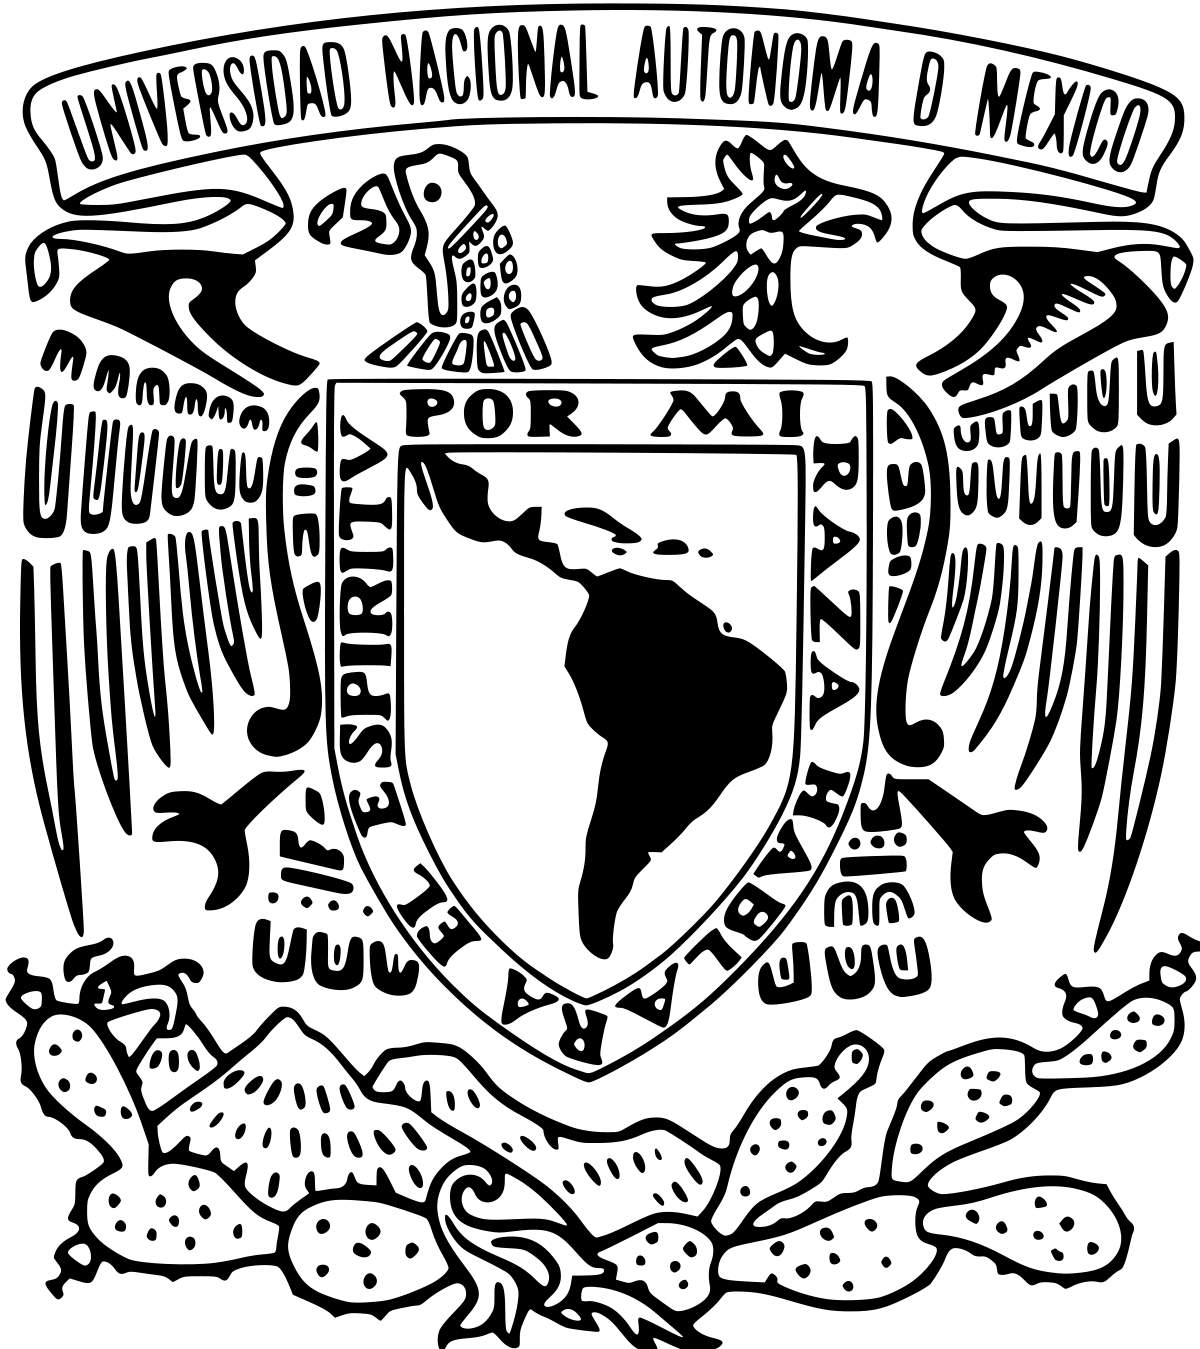
\includegraphics[height=3.4cm]{src/Img/Logo_UNAM.png}
    	\end{center}
    \end{minipage}\hfill
    \begin{minipage}{10cm}
    	\begin{center}
    	\textbf{\large Universidad Nacional Autónoma de México}\\[0.1cm]
        \textbf{Facultad de Ciencias}\\[0.1cm]
        \textbf{Análisis de Algoritmos  $|$ 7083}\\[0.1cm]
        Tarea 3 : $|$ Programacion Dinamica\\[0.1cm]
        Sosa Romo Juan Mario $|$ 320051926 \\[0.1cm]
        25/09/24
    	\end{center}
    \end{minipage}\hfill
    \begin{minipage}{3cm}
    	\begin{center}
    		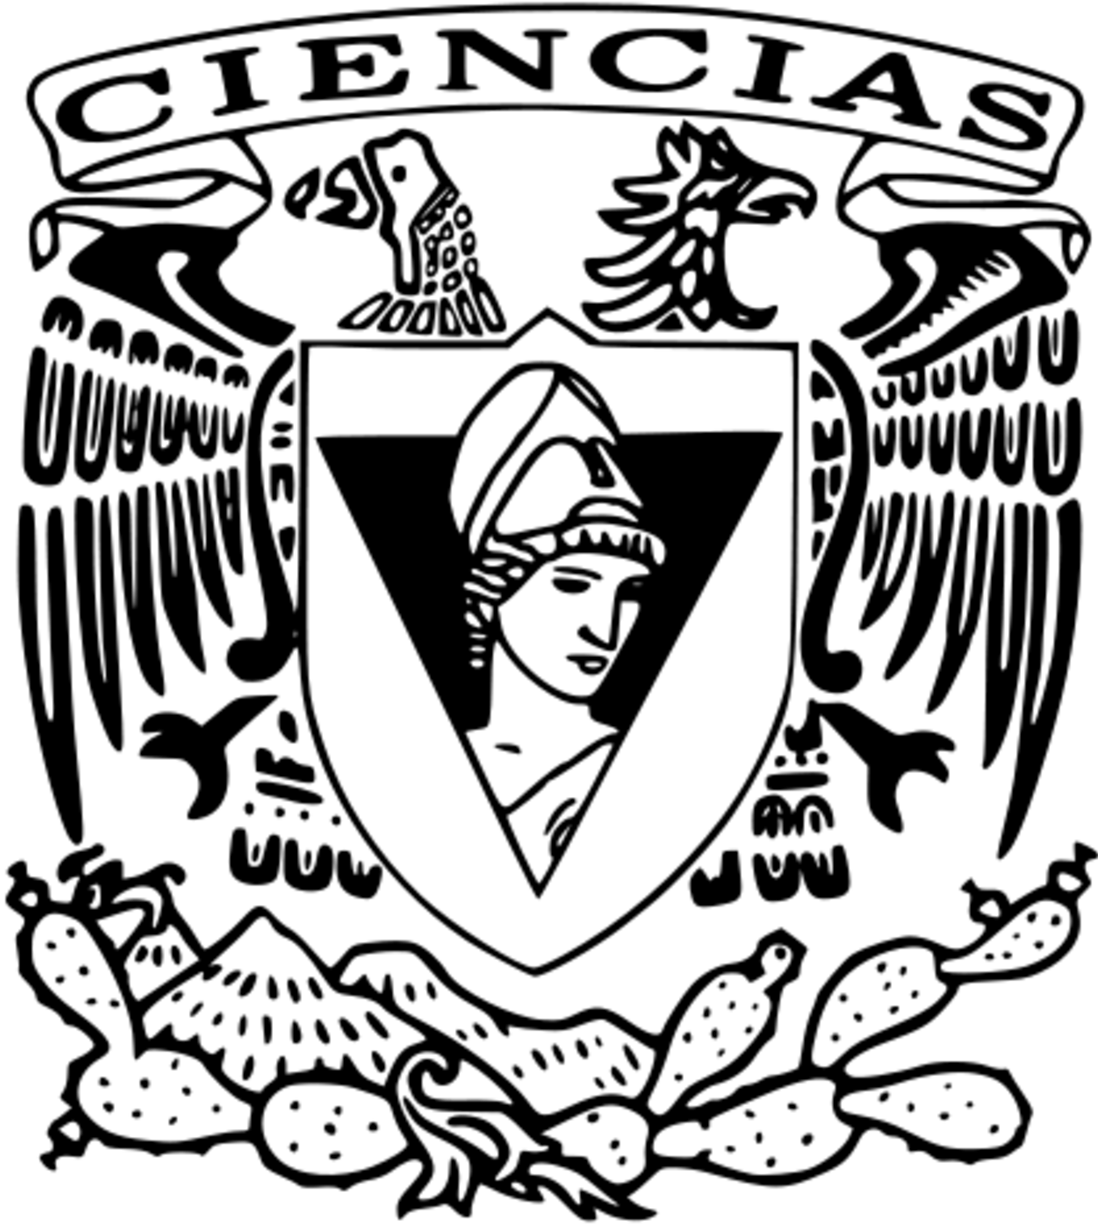
\includegraphics[height=3.4cm]{src/Img/Logo_FC.png}
    	\end{center}
    \end{minipage}
\end{center}


\rule{16.99cm}{0.1mm}

%------ Ejercicios -------- %
\begin{enumerate}
    \item \textbf{
    Un algoritmo glotón para regresar el cambio
    de n unidades usando el mínimo número de 
    monedas es el siguiente: Dar al cliente una
    moneda de mayor denominación, digamos d.
    Repite lo anterior para regresar el cambio 
    de n-d unidades.
}
\vspace{.3cm}

\textbf{
    Para cada una de las siguientes denominaciónes,
    determina si el algoritmo greedy antes mecionado
    mínimiza el número de monedas para dar el cambio.
    Si es así pruébalo, y si no lo es muestra un 
    contraejemplo.
}\vspace{.2cm}

\textcolor{red}{Esta probablemente no salio, si quiere no la califique pero la intente por si viene en el examen :v}
    \item \textbf{
    Construya el árbol de Huffman para codificar el siguiente texto:
    \begin{center}
        "El azote, hijo mío, se inventó para castigar afrontando al racional y para avivar la pereza del bruto que carece de razón; pero no para el niño decente y de vergüenza que sabe lo que le importa hacer y lo que nunca debe ejecutar, no amedrentado por el rigor del castigo, sino obligado por la persuasión de la doctrina y el convencimiento de su propio interés."
    \end{center}
}\vspace{.2cm}

No voy a explicar el algoritmo de Huffman, pues se vio en clase pero voy a hacer el procedimiento y luego mostrar con un árbol de Huffman online que esta bien hecho. \vspace{.2cm}

\textcolor{bibi}{Creamos el arbol de Huffman}
\begin{quote}
    \begin{itemize}
        \item \textbf{Paso 1:} Contamos la frecuencia de cada letra en el texto. (puede cambiar un poquito si consideras tabuladores o si yo conte mal xd)

        \begin{align*}
            \char`_ &: 65 \\
            e &: 39 \\
            a &: 34 \\
            o &: 27 \\
            r &: 25 \\
            n &: 21 \\
            i &: 17 \\
            l &: 15 \\
            t &: 13 \\
            d &: 13 \\
            c &: 12 \\
            p &: 11 \\
            s &: 9 \\
            u &: 9 \\
            v &: 5 \\
            g &: 5 \\
            z &: 4 \\
            , &: 4 \\
            m &: 4 \\
            y &: 4 \\
            b &: 4 \\
            q &: 4 \\
            \text{ó} &: 3 \\
            h &: 2 \\
            j &: 2 \\
            E &: 1 \\
            \text{í} &: 1 \\
            f &: 1 \\
            ; &: 1 \\
            \text{ñ} &: 1 \\
            \text{ü} &: 1 \\
            \text{é} &: 1 \\
            . &: 1 \\
        \end{align*}
        \item \textbf{Paso 2:} Creamos una lista con los nodos de cada letra y su frecuencia. (este paso literalmente solo es hacer eso entonces no muestro nada)
        \item \textbf{Paso 3:} Tomamos 2 arboles con las frecuencias mas bajas y los unimos en un nuevo arbol con la suma de las frecuencias, la raiz de este nuevo arbol es la suma de las frecuencias y los hijos son los arboles que unimos. Ademas, se etiqueta cada rama con un 0 si esta a la izquierda o un 1 si esta a la derecha, (este paso es el mas largo y tedioso, asi que solo muestro el resultado final)
        \item \textbf{Paso 4:} Repetimos el paso 3 hasta que solo quede un arbol. \vspace{.2cm}
    \end{itemize}

    No se si no se podia pero yo utilice un graficador en linea, igualmente el link del graficador es \href{https://www.csfieldguide.org.nz/en/interactives/huffman-tree/}{\underline{este}} y el resultado es este: \vspace{.2cm}

    \textbf{NOTA:} El graficador no le importa tanto si es izquierda o derecha al a hora de mostrar el resultado grafico (por eso aveces pone 0 a la derecha) pero internamente si lo esta haciendo solo lo dibuja al reves. \vspace{.2cm}
    \begin{center}
        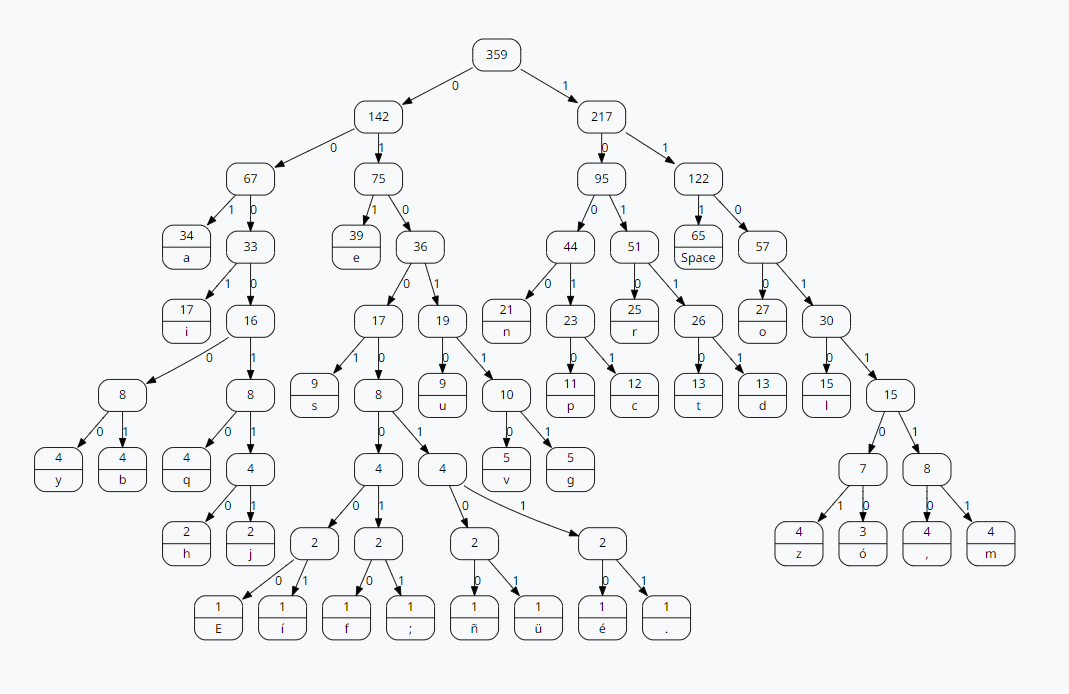
\includegraphics[width=14.9cm]{src/Img/ArbolHuffman.png}
    \end{center}

    Pero bueno por si acaso lo explico un poquito, hasta abajo vemos que los de frecuencia 1 se empezaron uniendo entre si generando arboles con raiz 2, a su vez se unieron entre si para generar arboles con raiz 4, aveces, cuando no hay arboles con la misma raiz, se toman los 2 de menor raiz digamos 8 y 9 se juntan para una raiz 17, y asi sucesivamente hasta que solo queda un arbol de raiz 359. \vspace{.2cm}

    Ahora, como mencionamos ir a la izquierda desde la raiz agrega un 0 a la codificacion del caracter y a la derecha un 1, entonces, si queremos saber la codificacion de una letra, simplemente seguimos el camino desde la raiz hasta la letra y anotamos los 0s y 1s que tomamos, este camino es unico aunque la codificacion no lo sea  (existen varias codificaciones de Huffman para este texto). Entonces por ejemplo el espacio tiene 111 como codificacion mientras que el . tiene una codificacion de 01000111 \vspace{.2cm} 
\end{quote}
    \item \textbf{Suponga que tenemos dos arreglos ordenados $A[1,\dots n]
\ y \ B[1, \dots, n]$ y un entero k. Describe un algoritmo para 
encontrar el \textit{k-ésimo} elemeneto en la unión de  \textit{A}
y \textit{B}. Por ejemplo, si $k=1$, tu algoritmo debe regresar el
elemento más pequeño de $A \cup B$; si $k=n$, tu algoritmo debe 
regresar la mediana de $A \cup B$. Puedes suponer que los arreglos 
no contienen duplicados. Tu algoritmo debe tener complejidad de tiempo
$\Theta (log \, n)$. Hint: Primero resuelve el caso especial k=n.}
    \begin{enumerate}
        \item \textbf{Show how to cover the board with $\frac{n \times n}{2}$ dominos.}\vspace{.2cm}

\textcolor{bibi}{}
\begin{quote}
\end{quote}
        \item \textbf{Remove the upper left and lower right corners from $B$. Show that you cannot cover the remaining board with $\frac{n \times n}{2}-1$ dominos.}\vspace{.2cm}

\textcolor{bibi}{Demostracion}
\begin{quote}
    Una manera medio rapida de ver esto es con un ejemplo, en este caso si por ejemplo tenemos un tablero 2x2, y quitamos las esquinas, nos queda la esquina superior derecha y la esquina inferior izquierda, y ahi no cabe un domino. \vspace{.2cm}

    Otro argumento para en general es ver la coloracion, si quitamos las esquinas, nos queda un tablero con $\frac{nxn}{2}-2$ cuadrados negros (podria ser blanco tambien pero el punto es que son del mismo color ya que las esquinas superior izquierda e inferior derecha estan en la misma diagonal porque n es par) y  $\frac{nxn}{2}$ cuadrados blancos y como los cuadrados tienen colores alternantes entonces cada domino cubre uno de cada tipo por lo que si no tienen la misma cantidad de colores no hay forma de cubrirlo. \vspace{.2cm}
\end{quote} 
        \item \textbf{Remove one arbitrary black square and one arbitrary white square from $B$. Show that the rest of the board can be covered with $\frac{n \times n}{2}-1$ dominos.}\vspace{.2cm}

\textcolor{red}{Esta no esta bien hecha no calificar xd}

\textcolor{bibi}{Demostracion por induccion}
\begin{quote}
    En este caso notamos que no se incumple lo de antes, es decir se mantienen la misma cantidad de cuadros de ambos colores por lo que por ahora podemos seguir. \vspace{.2cm}

    \textbf{Caso base: n=2}

    Para un tableror de 2x2 tenemos 2 de cada tipo, independientemente de cuales 2 quitemos nos queda o una fila o una columna de color alternante y se cubre con un domino o $\frac{2x2}{2}-1$. \vspace{.2cm}

    \textbf{Hipotesis de induccion: n}
    Para un tablero de $n \times n$ con $n$ par, si quitamos un cuadro de cada color, el tablero restante se puede cubrir con $\frac{n \times n}{2}-1$ dominos. \vspace{.2cm}

    \textbf{Paso inductivo: n+2}
    Tenemos un tablero de $(n+2) \times (n+2)$, quitamos un cuadro de cada color, ahora tomamos 2 filas y 2 columnas no afectadas por el cambio y las quitamos, nos queda un tablero de $n \times n$ y por hipotesis de induccion se puede cubrir con $\frac{n \times n}{2}-1$ dominos, ademas estas 2 filas y 2 columnas se pueden cubrir con lo que nos falta pero bueno ya no me da tiempo xd. \vspace{.2cm}
\end{quote}
    \end{enumerate}
    \item \textbf{Sea \textit{A} un arreglo de n númreos enteros distintos. Suponga
que \textit{A} tiene la siguiente propiedad: existe un indice $1 \leq k \leq
n$ tal que $A[1],\dots,A[k]$ es una secuencia incremental y $A[k+1],\dots,
A[n]$ es una secuencia decremental.}\\
    \item \textbf{Usted tiene que ordenar una serie $\Sigma_n$ de $n$ números, tales que todos son 0 ó 1. La única operación que puede hacer es comparar dos números cualesquiera $x$ y $y$, y cada que los compara recibe la respuesta $x < y$, $x = y$, or $x > y$.}\vspace{.2cm}
    \begin{enumerate}
        \item \textbf{De un algoritmo que con a lo más $n - 1$ comparaciones ordena $\Sigma_n$. Pruebe que su algoritmo es óptimo.}\vspace{.2cm}

\textcolor{bibi}{}
\begin{quote}
\end{quote}
        \item \textbf{Encuentre un algoritmo que utilizando en promedio $\frac{2n}{3}$ comparaciones ordena $\Sigma_n$ (esto bajo la suposición que los elementos de $\Sigma_n$ tienen la misma probabilidad de ser 0 ó 1). Demuestre que su algoritmo es óptimo.}\vspace{.2cm}

Algo vital para resaltar en este caso es que si tenemos información extra por lo que no significa que el algoritmo anterior no sea optimo. \vspace{.2cm}

\textcolor{bibi}{Usando arboles}
\begin{quote}
    La idea de este algoritmo va a ser agrupar por tipos cuando sean iguales y cuando no, ya tenemos un orden sobre esos grupos que sean diferentes; es importante destacar que en el caso que fueran todos de un solo tipo la complejidad sería $n - 1$ comparaciones. \vspace{.2cm}

    Vamos a comenzar por dividir nuestra serie de elementos en hojas de un arbol, adicionalmente a el valor que tengan (que desconocemos) vamos a agregarle un valor a estos nodos que indiquen de que tamaño es su grupo; ahora comparamos por pares (si nos sobra uno podemos compararlo en el siguiente nivel). Tenemos 4 casos posibles: \vspace{.2cm}

    \begin{enumerate}
        \item \textbf{$x=y$} Ambos son iguales (dos 1), en este caso creamos un nodo padre con el valor de uno de los 2 y el tamaño de su grupo es la suma del tamaño de ambos grupos (en este caso 2). \vspace{.1cm}
        \item \textbf{$x<y$} En este caso ya sabemos quienes son 1's y quienes son 0's, por lo que los contamos dependiendo del tamaño de su grupo y estos ya no juegan (sabemos que hay un 1 y un 0). \vspace{.1cm}
        \item \textbf{$x>y$} En este caso ya sabemos quienes son 1's y quienes son 0's, por lo que los contamos dependiendo del tamaño de su grupo y estos ya no juegan (sabemos que hay un 1 y un 0). \vspace{.1cm}
        \item \textbf{$x=y$} Ambos son iguales (dos 0), este caso es analogo al caso 1. \vspace{.2cm}
    \end{enumerate}

    Esto nos tomo $\mathbf{n/2}$ comparaciones, pero lo interesante aqui es que si todos los casos tienen la misma probabilidad (por la suposición del problema) entonces la mitad de los elementos ya estan ordenados y no los volvemos a comparar esto significa que en el siguiente nivel solo hay $(n/2)/2=n/4$ nodos (normalmente serían $n/2$ pero la mitad no sobrevive). \vspace{.2cm}

    Podemos repetir un procedimiento similar en el siguiente nivel, este tiene $n/4$ nodos por lo que comparando por parejas nos toma $(n/4)/2 = \mathbf{n/8}$ comparaciones. Seguimos haciendo esto y por ejemplo el siguiente nivel tendra $(n/8)/2=n/16$ nodos y usara $(n/16)/2=\mathbf{n/32}$ comparaciones. \vspace{.2cm}  

    Se sigue de este razonamiento que la cantidad de comparaciones se ve algo como esto: 
    \begin{align*}
        \frac{n}{2} + \frac{n}{4} + \frac{n}{8} + \cdots + 1 
    \end{align*}

    Esta es una progresión geométrica con razón de $\frac{1}{4}$ empezando por $\frac{n}{2}$, ademas en este caso cuando llegamos a la raiz mas bien no sabemos de que tipo es solo sabemos que todos sus elementos son del mismo tipo pero podrían ser 1's o 0's, por lo que ocupamos una comparación mas con alguno ya ordenado (si solo hay un tipo entonces ocupa $n-1$ comparaciones y esta trivialmente ordenado).
    \begin{align*}
        \frac{n/2}{1-1/4} = \frac{n/2}{3/4} = \frac{2n}{3}
    \end{align*}

    Hagamos un ejemplo grafico chico para ver como se ve esto: \vspace{.2cm}
    \begin{figure}[H]
        \centering
        \resizebox{1\textwidth}{!}{%
        \begin{circuitikz}
        \tikzstyle{every node}=[font=\LARGE]
        \draw  (3.75,7.75) circle (1cm) node {\LARGE 1,1} ;
        \draw  (6.25,7.75) circle (1cm) node {\LARGE 0,1} ;
        \draw  (8.75,7.75) circle (1cm) node {\LARGE 1,1} ;
        \draw  (11.25,7.75) circle (1cm) node {\LARGE 1,1} ;
        \draw  (13.75,7.75) circle (1cm) node {\LARGE 0,1} ;
        \draw  (16.25,7.75) circle (1cm) node {\LARGE 0,1} ;
        \draw  (18.75,7.75) circle (1cm) node {\LARGE 0,1} ;
        \draw  (21.25,7.75) circle (1cm) node {\LARGE 1,1} ;
        \node [font=\LARGE] at (12.25,5.5) {valor, tamaño de grupo};
        \draw  (5,10.25) circle (1cm) node {\LARGE null} ;
        \draw (3.75,8.75) to[short] (4.5,9.5);
        \draw (6.25,8.75) to[short] (5.5,9.5);
        \draw  (20,10.25) circle (1cm) node {\LARGE null} ;
        \draw (18.75,8.75) to[short] (19.5,9.5);
        \draw (21.25,8.75) to[short] (20.5,9.5);
        \draw  (10,10.25) circle (1cm) node {\LARGE 1,2} ;
        \draw (8.75,8.75) to[short] (9.5,9.5);
        \draw (11.25,8.75) to[short] (10.5,9.5);
        \draw  (15,10.25) circle (1cm) node {\LARGE 0,2} ;
        \draw (13.75,8.75) to[short] (14.5,9.5);
        \draw (16.25,8.75) to[short] (15.5,9.5);
        \draw  (12.5,14) circle (1cm) node {\LARGE null} ;
        \draw (10,11.25) to[short] (12,13.25);
        \draw (15,11.25) to[short] (13,13.25);
        \node [font=\LARGE] at (12.5,16) {\textbf{Final: [0,0,0,0,1,1,1,1]}};
        \node [font=\LARGE] at (1.25,9.25) {Me da un 1 y un 0};
        \node [font=\LARGE] at (17,12.5) {Me da dos 1 y dos 0};
        \node [font=\LARGE] at (23.75,9.25) {Me da un 1 y un 0};
        \end{circuitikz}
        }%
        \label{fig:ej5.2}
    \end{figure}

    En este caso tenemos 8 elementos, hacemos 4 comparaciones y ordenamos a 4; nos quedan 2 nodos vivos con lo que hacemos 1 comparación y tenemos 0 nodos vivos con lo que ya sabemos cuantos 1's y 0's hay. \vspace{.2cm}

    Notemos que no hay un caso terrible, en cuanto no sean iguales podemos quitar a todos los elementos de ambos arboles y como ya mencionamos el peor caso seria si todos fueran iguales. \vspace{.2cm}
\end{quote}
    \end{enumerate}
    \item \textbf{Se dice que un arreglo A[1,...,n] es k-ordenado si este puede ser dividido en k bloques cada uno de tamaño $\frac{n}{k}$ aproximadamente, tal que todos los elementos en cada bloque son mas grandes que el bloque anterior y mas pequeños que los elementos del bloque siguiente. Los elementos en cada bloque podrían no estar ordenados. Por ejemplo, el siguiente arreglo es 4-ordenado:
\begin{align*}
    1,2,4,3 \,|\, 7,6,5 \,|\, 10,11,9,12 \,|\, 15,13,16,14\\
\end{align*}}


    \begin{enumerate}
        \item \textbf{Describe un algoritmo que k-ordene un arreglo de tamaño n en tiempo $O(n \, logk)$.}\\

Para este problema vamos a utilizar una versión modificada de \textbf{Quick sort} pero además vamos a utilizar la versión que toma su pivote con la mediana en tiempo O(n) para asegurar la complejidad en el peor de los casos.\\

\textcolor{bibi}{Quick sort}
\begin{quote}
    Lo primero que nos interesa es que dividamos el arreglo en $k$ bloques, pero como estamos usando quick sort modificado, lo primero es encontrar la mediana en $O(n)$, una vez encontrada esta mediana tenemos un buen pivote, podemos comenzar a dividir, en este paso vamos a tener 2 fracciones de n, probablemente no estén cerca de ser $n/2$ pero si sabemos que serán algo como $n/c_1$ y $n/c_2$.\\

    En el siguiente paso, de nuevo buscamos la mediana en cada fracción en tiempo $O(n)$ y obtenemos de nuevo una fracción de n (asegurado por buscar la mediana); esto lo vamos a repetir hasta que el árbol llegue a arreglos de tamaño $n/k$ como lo estamos dividiendo en fracciones de $n$ entonces la altura del árbol binario implícito va a ser logarítmica, ahora vamos a checar cual es la altura de dicho árbol, en cada paso van a ser fracciones diferentes pero como queremos hacernos el calculo mas fácil en promedio podemos decir que se van a dividir en una fracción $1/c$ con c constante (en verdad c cambia en cada paso pero su valor es poco relevante). Entonces la altura del árbol la vamos a calcular de la siguiente manera, comenzamos con n elementos y luego vamos partiendo por nuestro c hasta que lleguemos a k grupos de tamaño $n/k$:
    \begin{align*}
        n, \frac{n}{c}, \frac{n}{c^2}, \dots, \frac{n}{c^m} = \frac{n}{k} \xrightarrow{} kn &= c^m * n \\
        k &= c^m \\
        log_c{\ k} &= log_c{\ c^m} \\
        log_c{\ k} &= m
    \end{align*}

    Notemos que los valores de C en realidad no alteran mas que la base del logaritmo y además m representaba el nivel de profundidad del árbol, es decir tras m niveles del árbol que dividía en fracciones de n tendremos k grupos de tamaño aproximado $n/k$.\\

    Entonces, sabemos que para cada nivel del árbol, buscaremos la mediana de las medianas que se puede hacer en $O(n)$ además de que vamos a recorrer todo el arreglo que también esta en $O(n)$; simplificando cada nivel hace una cantidad lineal de operaciones; después vimos que vamos a estar dividiendo (gracias a la mediana de las medianas) a n en una fracción de si misma por cada nivel y además dividiremos hasta que lleguemos a arreglos de tamaño $n/k$ de manera que tendremos $log_C(\ k)$ niveles, multiplicando estas complejidades tenemos que $O(n(log_C(\ k))) = O(n \ log(k))$, aunque hay que aclarar que las constantes ocultas probablemente son muy grandes especialmente estar calculando mediana de medianas en todos los pasos.\\
\end{quote}
        \item \textbf{What is a good strategy is $n$ is not known?}\vspace{.2cm}

\textcolor{bibi}{}
\begin{quote}
\end{quote}
    \end{enumerate}
    \item \textbf{Considera el siguiente algoritmo para ordenar:
\begin{center}
        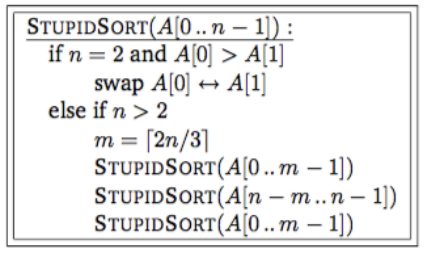
\includegraphics[width=5cm]{src/Img/stupidSort.png}\\
\end{center}}

    \item \textbf{Dado un arreglo $A$ con $n$ enteros positivos y negativos.}\vspace{.2cm}

\textcolor{bibi}{}
\begin{quote}
\end{quote}
    \begin{enumerate}
        \item \textbf{Suponiendo que puede cambiar de posición a las personas ¿Se puede resolver el problema con a lo mas una orden? Explique.}\\

Si, asumiendo que el mover de posición no cuenta como una orden, seria poner a todos los que tengan de una forma de un lado y los que lo tengan de la otra del lado contrario, así podríamos dar la orden de tomar uno de los 2 lados y pedirles a todos hasta el ultimo de esa forma que se cambien la gorra hacia el lado opuesto y tendríamos a todos de manera uniforme, (no se si entendí bien esta pregunta xd).\\
        \item \textbf{Dise\~na un algoritmo de programaci\'on din\'amica eficiente que determine si $Z$ es un \textit{shuffle} de $X$ y $Y$. \textit{Hint}: Los valores de la matriz de programaci\'on din\'amica que construyas, podr\'ian ser valores booleanos y no num\'ericos.}\vspace{.2cm}

El problema se parece bastante a la subcadena creciente mas grande.
La idea es usar una matriz de $|X|+1$ filas y $|Y|+1$ columnas, 
donde la celda $(i,j)$ indica si los primeros $i+j$ caracteres de $Z$
son un \textit{shuffle} de los primeros $j$ caracteres de $X$ y 
los primeros $i$ caracteres de $Y$. (podemos cambiar cual es quien pero asi lo hice) \vspace{.2cm}
    
\textcolor{bibi}{Usando matriz y programaci\'on din\'amica:}\vspace{.2cm}
\begin{quote}

    Podemos empezar verificando que $|X|+|Y|=|Z|$, si no es asi entonces
    no puede ser un \textit{shuffle} de $X$ y $Y$. \vspace{.2cm}

    Tenemos entonces que nuestra matriz se va a ver algo as\'i:

    \begin{table}[H]
        \centering
        \begin{tabular}{lllllll}
                &                              &                       & $x_0$                 & $x_1$                 & $\dots$               & $x_n$                 \\
                & i/j                          & 0                     & 1                     & 1                     & $\dots$               & n                     \\ \cline{3-7} 
                & \multicolumn{1}{l|}{0}       & \multicolumn{1}{l|}{1} & \multicolumn{1}{l|}{} & \multicolumn{1}{l|}{} & \multicolumn{1}{l|}{} & \multicolumn{1}{l|}{} \\ \cline{3-7} 
        $y_0$   & \multicolumn{1}{l|}{1}       & \multicolumn{1}{l|}{} & \multicolumn{1}{l|}{} & \multicolumn{1}{l|}{} & \multicolumn{1}{l|}{} & \multicolumn{1}{l|}{} \\ \cline{3-7} 
        $y_1$   & \multicolumn{1}{l|}{2}       & \multicolumn{1}{l|}{} & \multicolumn{1}{l|}{} & \multicolumn{1}{l|}{} & \multicolumn{1}{l|}{} & \multicolumn{1}{l|}{} \\ \cline{3-7} 
        $\dots$ & \multicolumn{1}{l|}{$\dots$} & \multicolumn{1}{l|}{} & \multicolumn{1}{l|}{} & \multicolumn{1}{l|}{} & \multicolumn{1}{l|}{} & \multicolumn{1}{l|}{} \\ \cline{3-7} 
        $y_m$   & \multicolumn{1}{l|}{m}       & \multicolumn{1}{l|}{} & \multicolumn{1}{l|}{} & \multicolumn{1}{l|}{} & \multicolumn{1}{l|}{} & \multicolumn{1}{l|}{} \\ \cline{3-7} 
        \end{tabular}
    \end{table}

    Ahora vamos a ver como llenarla, primero por la definición que hicimos, el indice
    (i,j) sera 1 pues los primeros 0+0 caracteres de Z siempre seran shuffle de los primeros
    0 caracteres de X y los primeros 0 caracteres de Y. \vspace{.2cm}

    Para la primera fila, hay que checar que los primeros $j$ caracteres de $X$ sean iguales
    a los primeros $j$ caracteres de $Z$, si es asi, entonces la celda $(0,j)$ sera 1, si no
    entonces sera 0; para checar esto podemos checar si el caracter j es igual en ambos y despues
    checar si a la izquierda ya tenemos un 1. ( esto es equivalente a: M[0][j]=M[0][j-1] AND X[j-1]==Z[j-1]
    tenemos que restar 1 porque las cadenas tienen indice en 0 pero tambien lo puedes entender con cantidad
    de caracteres) \vspace{.2cm}

    Para la primera columna, es lo mismo que la fila pero con $Y$ y $Z$, esto se puede entender como
    M[i][0]=M[i-1][0] AND Y[i-1]==Z[i-1]. \vspace{.2cm}

    Ahora para el caso de en medio hay que checar que los primeros $i+j$ caracteres de $Z$ sean shuffle
    de los primeros $j$ caracteres de $X$ y los primeros $i$ caracteres de $Y$, esto se puede entender
    como M[i][j]=M[i-1][j] AND Y[i-1]==Z[i+j-1] OR M[i][j-1] AND X[j-1]==Z[i+j-1]. \vspace{.2cm}

    De manera general nuestra funcion quedaria algo asi:
    \scriptsize
    \begin{align*}
        M[i][j]=\begin{cases}
            1 & \text{si } i=0 \text{ y } j=0 \\
            (M[i-1][j] \text{ AND } Y[i-1]==Z[i+j-1]) \text{ OR } (M[i][j-1] \text{ AND } X[j-1]==Z[i+j-1]) & \text{si } i>0 \text{ y } j>0 \\
        \end{cases}
    \end{align*}

    Al final sabremos si $Z$ es un \textit{shuffle} de $X$ y $Y$ si $M[|Y|][|X|]=1$, ademas el camino
    para ir de la celda $(|Y|,|X|)$ a la celda $(0,0)$ nos dira cuales son los caracteres que se usaron. \vspace{.2cm}

    Este algoritmo tiene complejidad $O(|X|*|Y|)$ y usa $O(|X|*|Y|)$ memoria, esto pues la matriz es de tamaño
    $(|X|+1)*(|Y|+1)$ y se llena en cada celda una vez tomando $O(1)$ tiempo (checar arriba y abajo, tomar un indice de 
    una cadena y compararlo con el indice en otra cadena que puede ser O(1)). \vspace{.2cm}

    Para entender mejor checar el ejemplo de arriba.
\end{quote}


\newpage
        \item \textbf{Suponiendo que no puede cambiar de posición a las personas. Diseñe un algoritmo de tiempo lineal tal que todos los asistentes tengan la visera del mismo lado al ingresar pero garantice el mínimo numero de cambios.}\\

En este caso primero vamos a contar la cantidad que lo tiene de cada forma, (de nuevo no se si contamos esto como algo pero sube la complejidad implementándolo) esto ocupa 0 ordenes o cambios, una vez contado esto solo hay que recorrer la lista y pedirles a los que tuvieron la forma menos común, que se giren la gorra.
    \end{enumerate}
    \item \textbf{Suppose that we are given a sequence of $n$ values $x_1, x_2, \dots, x_n$ and seek to quickly answer repeated queries of the form: given $i$ and $j$, find the smallest value in $x_i, \dots, x_j$.}\vspace{.2cm}

Como nota importante para este problema es que no nos sirve ordenar el arreglo puesto que esto cambia la posición de los elementos y no podemos acceder al rango especifico. \vspace{.2cm}
    \begin{enumerate}
        \item \textbf{Design a data structure that uses $O(n^2)$ space and answers queries in $O(1)$ time.}\vspace{.2cm}

\textcolor{bibi}{}
\begin{quote}
\end{quote}
        \item \textbf{Design a data structure that uses $O(n)$ space and answers queries in $O(log \ n)$ time.}\vspace{.2cm}

\textcolor{bibi}{Segment Tree}
\begin{quote}
    La idea es usar un segment tree para guardar los minimos de los rangos. Comenzamos por dividir el arrreglo en subarrerglos, cada nodo en el segment tree representa el minimo de un intervalo en el arreglo original. (vamos a guardar 2 indices tambien para saber que intervalo cubre) \vspace{.2cm}

    La raiz del arbol representa el rango completo $[1, n]$ y por tanto el minimo de todo el arreglo. Cada nodo tiene dos hijos que representan la mitad del rango del padre y tienen el minimo de ese rango. \vspace{.2cm}

    El razonamiento del porque este arbol usa $O(n)$ espacio es que el rango se va partiendo a la mitad y por tanto el arbol tiene a lo mucho $2n$ nodos donde cada nodo solo guarda 3 numeros. (serie geometica con termino inicial n y razon $1/2$). \vspace{.2cm}

    Para construir el arbol, tomamos el arreglo y lo dividimos en 2 partes, si no es de tamaño 1, llamamos recursivamente a la funcion para cada parte y guardamos el minimo de cada parte en el nodo actual la altura de este arbol sera de $O(\log \ n)$ y construirlo toma O(n). \vspace{.2cm}

    Para responder a las queries, si el rango del nodo actual esta contenido en el rango de la query, devolvemos el minimo de ese rango. Si el rango del nodo actual esta fuera del rango de la query, lo ingoramos. Si el rango del nodo actual intersecta con el rango de la query, llamamos recursivamente a los hijos y devolvemos el minimo de los minimos de los hijos, esto toma $O(\log \ n)$ pues en cada nivel procesamos a lo mas 2 nodos (un rango es continuo) y la altura del arbol es $O(\log \ n)$. \vspace{.2cm}
\end{quote}
    \end{enumerate}
    \item \textbf{
    Diseña un algoritmo de tiempo $O(|V|+|E|)$ determine si una gráfica dirigida 
    $G = (V,E)$ contiene o no un ciclo.
}\vspace{.2cm}

\textcolor{bibi}{DFS Modificado}
\begin{quote}
    Para determinar si una gráfica dirigida $G = (V,E)$ contiene un ciclo, se 
    puede utilizar una modificación del algoritmo de búsqueda en profundidad 
    (DFS). \vspace{.2cm}

    El algoritmo de DFS primero que nada consiste en recorrer todos los nodos 
    utilizando una pila. Empezando por un nodo, lo agregamos a la pila, lo sacamos
    marcamos como visitado (podemos usar un arreglo booleano o mas facil agregarle informacion a los vertices, tipo (valor, visitado, listaAdyacencias)) y agregamos su lista de adyacencias a la pila. Despues vamos sacando del tope, si el nodo no ha sido visitado, lo marcamos como visitado y repetimos con su lista de adyacencias, escencialmente visitando a lo mas profundo que podemos antes de visitar a sus vecinos, este algoritmo tiene complejidad de $O(|V|+|E|)$ cada vertice se visita solo una vez pues se marca como visitado y todas las aristas se visitan pues cuando checamos un nodo tenemos que ver a todos sus vecinos para saber si ya estan o no checados. \vspace{.2cm}

    Para determinar si una gráfica dirigida $G = (V,E)$ contiene un ciclo, se
    puede utilizar una modificación del algoritmo de DFS. La modificación consiste
    en agregar un arreglo de booleanos que nos indique si un nodo ha sido visitado
    en el recorrido actual (podemos buscar a un nodo por su indice), la idea es la misma, ir marcando vertices pero esta vez solo vamos a ir marcando el recorrido actual y cuando hagamos backtrack tambien quitamos esos nodos de la lista de visitados. Si en algun momento encontramos un nodo que ya ha sido visitado en el recorrido actual, entonces hemos encontrado un ciclo. \vspace{.2cm}

    Como el algoritmo de DFS tiene complejidad $O(|V|+|E|)$, la modificación, solo tiene que agregar un arreglo de booleanos que tiene complejidad $O(|V|)$, por lo que la complejidad del algoritmo modificado se queda en $O(|V|+|E|)$. \vspace{.2cm}

    Se puede justificar que funciona pues si existe un camino que contenga un ciclo entonces en algun momento vamos a visitar un nodo que ya habiamos visitado en el recorrido actual, ademas, el no revisitar nodos que ya han sido visitados en el recorrido actual podria parecer que podria no dejarnos ver ciclos pero como estamos usando DFS si el ciclo existe por debajo de un nodo ya visitado entonces lo habriamos cachado en ese otro recorrido y no hay necesidad de volver a visitarlo. 
\end{quote}
    \item \textbf{Let $G = (V, E)$ be a bipartite graph with vertex partition $V = L \cup R$, and let $G'$ be its corresponding flow network. Give a good upper bound on the length of any augmenting path found in $G'$ during the execution of FORD-FULKERSON.}\vspace{.2cm}

\textcolor{bibi}{}
\begin{quote}
\end{quote}
    \item \textbf{Professor Adams has two children who, unfortunately, dislike each other. The problem is so severe that not only do they refuse to walk to school together, but in fact each one refuses to walk on any block that the other child has stepped on that day. The children have no problem with their paths crossing at a corner. Fortunately both the professor’s house and the school are on corners, but beyond that he is not sure if it is going to be possible to send both of his children to the same school. The professor has a map of his town. Show how to formulate the problem of determining if both his children can go to the same school as a maximum-flow problem.}\vspace{.2cm}

\textcolor{bibi}{}
\begin{quote}
\end{quote}
    \item \textbf{Mientras caminas por la playa encuentras un cofre de tesoros. El cofre contiene $n$ tesoros con pesos $w_1, \dots, w_n$ y valores $v_1, \dots, v_n$. Desafortunadamente sólo tienes una mochila que solo tiene capacidad de carga $M$. Afortunadamente los tesoros se pueden romper si es necesario. Por ejemplo, la tercera parte de un tesoro $i$ tiene peso $\frac{w_i}{3}$ y valor $\frac{v_i}{3}$.}\vspace{.2cm}

\textcolor{bibi}{}
\begin{quote}
\end{quote}
    \begin{enumerate}
        \item \textbf{Describe un algoritmo voraz de tiempo $\Theta(n log n)$ que resuelve este problema.}\vspace{.2cm}

\textcolor{bibi}{}
\begin{quote}
\end{quote}
        \item \textbf{Prueba que tu algoritmo obtiene la solución correcta.}\vspace{.2cm}

\textcolor{bibi}{}
\begin{quote}
\end{quote}
        \item \textbf{Mejora el tiempo de ejecución de tu algoritmo a $\Theta(n)$}\vspace{.2cm}

La verdad no estoy seguro de esta parte pero lo voy a intentar:

\textcolor{bibi}{Usando K-select}
\begin{quote}
    La idea para esta variación de la solución empieza igual, tomamos y obtenemos la relación valor peso (densidad) para cada objeto. Pero en vez de ordenar completamente el arreglo usaremos selection k para considerar solo una parte del arreglo, una cosa importante en este algoritmo es que para mantener su complejidad en $O(n)$ voy a usar la mediana de medianas para seleccionar el pivote, esto me garantiza que el algoritmo no se vaya a $O(n^2)$. \vspace{.2cm}

    Una vez tomando la mediana de medianas en $O(n)$ hacemos 3 particiones del arreglo, los elementos menores a la mediana, los iguales y los mayores; ahora calculamos la suma de los pesos de los elementos cuya densidad es mayor a la mediana, si esta suma es igual a la capacidad de la mochila entonces terminamos y nos podemos llevar solo a esos. \vspace{.2cm}

    Si la suma es menor a la capacidad de la mochila, vamos calculando los pesos de los objetos cuya densidad es igual a la mediana y viendo si nos van cabiendo en la mochila hasta que se llene, si se llena acabamos. \vspace{.2cm}

    Si aun no se llena, entonces calculamos la mediana de medianas para los menores y repetimos el proceso. \vspace{.2cm}

    Otro caso que puede pasar es que la suma de los pesos de los objetos cuya densidad es mayor a la mediana sea mayor a la capacidad de la mochila, en este caso calculamos la mediana de medianas para los mayores y repetimos el proceso. \vspace{.2cm}

    Si en algun paso estamos en una particion y solo cabe una fraccion de un objeto, entonces lo tomamos y terminamos. \vspace{.2cm}

    Me parece que este algoritmo tiene una complejidad de $O(n)$, estamos haciendo $O(n)$ operaciones por paso y en cada paso reducimos el tamaño del arreglo a la mitad, la serie tiende a algo en $O(n)$.
\end{quote}
    \end{enumerate}
    \item \textbf{Encuentre la parentización óptima para multiplicar seis matrices de dimensiones $4 \times 9$, $9 \times 4$, $4 \times 10$, $10 \times 2$, $2 \times 5$, $5 \times 6$.}\vspace{.2cm}

Primero que nada voy a ponerle nombres a las matrices con las que estoy trabajando para que sea más fácil referirse a ellas. Así que las matrices serán:

\begin{align*}
    A0 & : 4 \times 9 \\
    A1 & : 9 \times 4 \\
    A2 & : 4 \times 10 \\
    A3 & : 10 \times 2 \\
    A4 & : 2 \times 5 \\
    A5 & : 5 \times 6   
\end{align*}

Y el vector de dimensiones será $p = \{4, 9, 4, 10, 2, 5, 6\}$. \vspace{.2cm}

\textcolor{bibi}{Usando DP}
\begin{quote}
    Voy a crear una matriz $dp$ de tamaño $6 \times 6$ donde $dp[i][j]$ va a ser el costo mínimo de multiplicar las matrices $A_i \times A_{i+1} \times \ldots \times A_j$. \vspace{.2cm}

    Además, voy a crear una matriz $s$ de tamaño $6 \times 6$ donde $s[i][j]$ va a ser el índice de la matriz que se va a multiplicar en la última multiplicación de la cadena $A_i \times A_{i+1} \times \ldots \times A_j$. \vspace{.2cm}

    Para llenar la matriz $dp$ y $s$ voy a usar la siguiente función:
    \begin{align*}
        \begin{cases}
            \text{dp}[i][j] &= \min_{i \leq k < j} \{ \text{dp}[i][k] + \text{dp}[k+1][j] + p_{i} \cdot p_{k+1}\cdot p_{j+1} \} \quad \text{si } i < j \\
            \text{dp}[i][j] &= 0 \quad \text{si } i = j
        \end{cases} \\
    \end{align*}

    Donde $p_{i-1} \cdot p_k \cdot p_j$ es el numero de operaciones que se hacen al multiplicar las matrices resultantes de esas subcadenas. \vspace{.2cm}

    Y para llenar la matriz $s$ voy a usar la siguiente función:
    \begin{align*}
        \text{s}[i][j] = k
    \end{align*}

    Empezamos por llenar la tabla $dp$ por su diagonal, es decir, $dp[i][i] = 0$ para todo $i$ esto es porque el costo mínimo de multiplicar una sola matriz es 0, despues seguimos la función es optimo ir llendo en diagonales empezando por la principal para arriba, podemos optimizar y solo llenar la mitad de la matriz ya que es simétrica. \vspace{.2cm}

    Ahora si vamos a aplicarlo y llenar la tabla (cuidado con confundir indices y elementos): \vspace{.2cm}

    \begin{center}
        % Tabla de costos (dp)
        \noindent
        \textbf{Tabla de costos mínimos (dp)} \\
        \begin{tabular}{c|*{6}{c}}
        i/j & $0$ & $1$ & $2$ & $3$ & $4$ & $5$ \\
        \hline
        $0$ &  0  & 144 & 304 & 224 & 264 & 332 \\
        $1$ &     &  0  & 360 & 152 & 242 & 320 \\
        $2$ &     &     &  0  & 80  & 120 & 188 \\
        $3$ &     &     &     &  0  & 100 & 180 \\
        $4$ &     &     &     &     &  0  & 60  \\
        $5$ &     &     &     &     &     & 0   \\
        \end{tabular}

        \vspace{1cm}

        % Tabla de divisiones (s)
        \noindent
        \textbf{Tabla de puntos de división (s)} \\
        \begin{tabular}{c|*{6}{c}}
        i/j & $0$ & $1$ & $2$ & $3$ & $4$ & $5$ \\
        \hline
        $0$ &  0  &  0  &  1  &  0  &  3  &  3  \\
        $1$ &     &  0  &  1  &  1  &  3  &  3  \\
        $2$ &     &     &  0  &  2  &  3  &  3  \\
        $3$ &     &     &     & 0   &  3  &  3  \\
        $4$ &     &     &     &     &  0  &  4  \\
        $5$ &     &     &     &     &     &  0  \\
        \end{tabular}
    \end{center}

    No escribi todos los calculos para no hacerlo tan largo pero es un proceso tedioso y cada uno de los valores puede cambiar dependiendo del k en el que vamos. \vspace{.2cm}

    Como vemos el costo minimo es 332 y el punto de división es 3, eso significa que creamos un grupo con las matrices $A_0, A_1, A_2,A_3$ y otro con las matrices $A_4, A_5$ nos queda $(A_0, A_1,$ $ A_2,A_3)$ $(A_4$, $ A_5)$ hasta ahora. \vspace{.2cm} 

    Checamos $s[0,3]=0$ asi que el primer grupo se divide en $(A_0$ $(A_1, A_2,A_3))$ y el segundo grupo se queda igual. \vspace{.2cm}  

    Checamos $s[1,3]=1$ asi que el primer grupo se divide en $(A_0$ $(A_1$ $(A_2,A_3)))$ y el segundo grupo se queda igual, separar mas este grupo ya no tiene mucho efecto porque se queda igual. \vspace{.2cm}

    Seguimos con el segundo grupo pero igual ya solo son 2 matrices entonces lo dejamos asi, al final nos queda la siguiente parentización óptima: $$(A_0 \times (A_1 \times (A_2 \times A_3))) \times (A_4 \times A_5)$$ \vspace{.2cm}
\end{quote}

    \item \textbf{Sea $P_n$ una familia de $n$ puntos en el plano, en posición general. Encuentre un algoritmo que encuentre el triángulo de mayor área cuyos vértices estén en $P_n$. Su algoritmo tiene que trabajar en menos de $O(n^3)$. Hint: Pruebe primero que los vértices de dicho triángulo están en el cierre convexo de $P_n$, esto reduce el problema al caso en que los elementos de $P_n$ son los vértices de un polígono convexo.}\vspace{.2cm}

\textcolor{bibi}{}
\begin{quote}
\end{quote}
    \item \textbf{Supongamos que usted es el dueño de la compañía Anuncios Espectaculares y que recibe un contrato para colocar anuncios espectaculares en la autopista México Querétaro . Los lugares donde puede colocar sus anuncios están localizados en los kilómetros ${ x_1, \dots , x_n }$ de dicha autopista. Si usted coloca un anuncio en el lugar localizado en el kilómetro $x_i$, recibirá una ganancia $r_i$. Por razones de seguridad, los anuncios no pueden estar muy cerca uno del otro, y la distancia entre dos anuncios consecutivos tiene que ser al menos 10 kilómetros. Observe que la distancia entre dos sitios cualquiera donde puede localizar sus anuncios no es necesariamente mayor que 10 kilómetros. }

\textbf{Encuentre un algoritmo que resuelva el problema de colocar anuncios de tal forma que las ganancias de su compañía se maximicen. Por ejemplo si:}

$$\{x_1, x_2, x_3, x_4\} = \{12, 14, 23, 28\}$$
    y
$$\{r_1, r_2, r_3, r_4\} = \{5,6,5,1\}$$

\textbf{la solución óptima sería colocar anuncios en los kilómetros 12 y 24 para una ganancia de 10.}\vspace{.2cm}

\textcolor{bibi}{}
\begin{quote}
\end{quote}
    \item \textbf{Consider the following data compression technique. We have a table of $m$ text strings, each at most $k$ in length. We want to encode a data string $D$ of length $n$ using as few text strings as possible. For example, if our table contains $(a,a,abab,b)$ and the data string is $bababbaababa$, the best way to encode it is $(b,abab,ba,abab,a)$ a total of five code words. Give an $O(nmk)$ algorithm to find the length of the best encoding. You may assume that every string has at least one encoding in terms of the table.}\vspace{.2cm}

Un detalle muy importante en esta parte es que no nos piden regresar el código, sino la longitud del mejor código. Por lo tanto, no es necesario guardar los códigos, sino simplemente la longitud de los mismos. \vspace{.2cm}

\textcolor{bibi}{Usando DP}
\begin{quote}
    Comenzamos definiendo un arreglo $dp$ de tamaño $n+1$ donde $dp[i]$ será el minimo numero de palabras necesarias para codificar los primeros $i$ caracteres de $D$. Inicializamos $dp[0] = 0$ (0 palabras para codificar la cadena vacia). \vspace{.2cm}
    
    Ahora inicia lo interesante, para cada posicion $i$ de $D$ y para cada palabra en la tabla digamos $s$ vamos a checar si $s$ es sufijo de $D$ de 0 a $i$ es importante notar que la longitud de las palabras es a lo mas $k$, si $s$ es sufijo entonces sea $j = i - |s|$ y updateamos el arreglo de la siguiente manera: $$dp[i]=min(dp[i],dp[j]+1)$$ Lo que estamos intentando hacer aqui basicamente es codificar los primeros j caracteres de $D$ y luego agregar la palabra $s$ para codificar los primeros $i$ caracteres de $D$ para ver si nos da menos palabras que codificar los primeros $i$ caracteres de $D$ directamente. Finalmente la respuesta sera $dp[n]$. \vspace{.2cm}

    Ademas de esto nuestra funcion de recurencia le agregamos valores por defecto para poder usar la funcion min, $dp[i]=\infty \ ;  \forall i>0$ \vspace{.2cm}

    \textbf{Complejidad:} La complejidad de este algoritmo es $O(nmk)$ ya que tenemos que recorrer cada posicion de $D$ (n) y para cada posicion tenemos que recorrer cada palabra de la tabla (m) y para cada palabra tenemos que recorrer la palabra para ver si es sufijo de $D$ (k).

    Para nuestro ejemplo, corri un codigo en python y obtuve la siguiente los $dp$ en cada iteracion:

    $$
    \begin{array}{|c|c|c|c|c|c|c|c|c|c|c|c|c|}
        \hline
        0 & 1 & \infty & \infty & \infty & \infty & \infty & \infty & \infty & \infty & \infty & \infty & \infty \\
        \hline
        0 & 1 & 1 & \infty & \infty & \infty & \infty & \infty & \infty & \infty & \infty & \infty & \infty \\
        \hline
        0 & 1 & 1 & 2 & \infty & \infty & \infty & \infty & \infty & \infty & \infty & \infty & \infty \\
        \hline
        0 & 1 & 1 & 2 & 2 & \infty & \infty & \infty & \infty & \infty & \infty & \infty & \infty \\
        \hline
        0 & 1 & 1 & 2 & 2 & 2 & \infty & \infty & \infty & \infty & \infty & \infty & \infty \\
        \hline
        0 & 1 & 1 & 2 & 2 & 2 & 3 & \infty & \infty & \infty & \infty & \infty & \infty \\
        \hline
        0 & 1 & 1 & 2 & 2 & 2 & 3 & 3 & \infty & \infty & \infty & \infty & \infty \\
        \hline
        0 & 1 & 1 & 2 & 2 & 2 & 3 & 3 & 4 & \infty & \infty & \infty & \infty \\
        \hline
        0 & 1 & 1 & 2 & 2 & 2 & 3 & 3 & 4 & 5 & \infty & \infty & \infty \\
        \hline
        0 & 1 & 1 & 2 & 2 & 2 & 3 & 3 & 4 & 5 & 5 & \infty & \infty \\
        \hline
        0 & 1 & 1 & 2 & 2 & 2 & 3 & 3 & 4 & 5 & 5 & 4 & \infty \\
        \hline
        0 & 1 & 1 & 2 & 2 & 2 & 3 & 3 & 4 & 5 & 5 & 4 & 5 \\
        \hline
    \end{array}
    $$ \vspace{.2cm}

    Donde la respuesta es 5, nos da 12 iteraciones porque la longitud de $D$ es 12, en cada iteracion tuvo que checar toda la tabla de palabras y para cada palabra tuvo que recorrer la palabra para ver si era sufijo de $D$. \vspace{.2cm}
\end{quote}
    \item \textbf{La compañía \textit{Monsters, Inc} preparó para el día de hoy una fila de $n \geq 2$ puertas para abrir y recolectar los gritos de los niños con el fin de abastecer de energía a la Monstropolis. Con el propósito de salir temprano los monstruos determinaron abrir todas las puertas de jalón y así terminar lo más rápido posible, por lo que asignaron a Sullivan a recorrer toda la fila y abrir todas las puertas. Al ver el desastre que esto causaría, Mike Wazowski recorrió la fila y cerró todas las puertas de manera alternada iniciando en la puerta 2. Sin embargo, ¡Quedaron $\frac{n}{2}$ puertas abiertas!. Por lo que el resto de los monstruos decidieron ayudar de la siguiente manera: el monstruo con el recorrido i-ésimo, cambiaría el estado de cada i-ésima puerta iniciando desde la puerta i. Después de hacer este proceso $n$ veces, ¿Quedan puertas abiertas? ¿Cuántas y cuáles son si es el caso?}\vspace{.2cm}

Este problema es mas de teoría de números aunque tambien se puede programar para ver casos específicos.

\textcolor{bibi}{Usando teoria de números}
\begin{quote}
    Para empezar hice un ejemplo a mano para darme una idea de como se comportaba el problema. En este caso $n=26$.
    \begin{align*}
        [0,0,0,0,0,0,0,0,0,0,0,0,0,0,0,0,0,0,0,0,0,0,0,0,0,0] \\
    2 \ [0,1,0,1,0,1,0,1,0,1,0,1,0,1,0,1,0,1,0,1,0,1,0,1,0,1] \\
    3 \ [0,1,1,1,0,0,0,1,1,1,0,0,0,1,1,1,0,0,0,1,1,1,0,0,0,1] \\
    4 \ [0,1,1,0,0,0,0,0,1,1,0,1,0,1,1,0,0,0,0,0,1,1,0,1,0,1] \\
    5 \ [0,1,1,0,1,0,0,0,1,0,0,1,0,1,0,0,0,0,0,1,1,1,0,1,1,1] \\
    6 \ [0,1,1,0,1,1,0,0,1,0,0,0,0,1,0,0,0,1,0,1,1,1,0,0,1,1] \\
    7 \ [0,1,1,0,1,1,1,0,1,0,0,0,0,0,0,0,0,1,0,1,0,1,0,0,1,1] \\
    8 \ [0,1,1,0,1,1,1,1,1,0,0,0,0,0,0,1,0,1,0,1,0,1,0,1,1,1] \\
    9 \ [0,1,1,0,1,1,1,1,0,0,0,0,0,0,0,1,0,0,0,1,0,1,0,1,1,1] \\
    10 \ [0,1,1,0,1,1,1,1,0,1,0,0,0,0,0,1,0,0,0,0,0,1,0,1,1,1] \\
    11 \ [0,1,1,0,1,1,1,1,0,1,1,0,0,0,0,1,0,0,0,0,0,0,0,1,1,1] \\
    12 \ [0,1,1,0,1,1,1,1,0,1,1,1,0,0,0,1,0,0,0,0,0,0,0,0,1,1] \\
    13 \ [0,1,1,0,1,1,1,1,0,1,1,1,1,0,0,1,0,0,0,0,0,0,0,0,1,0] \\
    14 \ [0,1,1,0,1,1,1,1,0,1,1,1,1,1,0,1,0,0,0,0,0,0,0,0,1,0] \\
    15 \ [0,1,1,0,1,1,1,1,0,1,1,1,1,1,1,1,0,0,0,0,0,0,0,0,1,0] \\
    16 \ [0,1,1,0,1,1,1,1,0,1,1,1,1,1,1,0,0,0,0,0,0,0,0,0,1,0] \\
    17 \ [0,1,1,0,1,1,1,1,0,1,1,1,1,1,1,0,1,0,0,0,0,0,0,0,1,0] \\
    18 \ [0,1,1,0,1,1,1,1,0,1,1,1,1,1,1,0,1,1,0,0,0,0,0,0,1,0] \\
    19 \ [0,1,1,0,1,1,1,1,0,1,1,1,1,1,1,0,1,1,1,0,0,0,0,0,1,0] \\
    20 \ [0,1,1,0,1,1,1,1,0,1,1,1,1,1,1,0,1,1,1,1,0,0,0,0,1,0] \\
    21 \ [0,1,1,0,1,1,1,1,0,1,1,1,1,1,1,0,1,1,1,1,1,0,0,0,1,0] \\
    22 \ [0,1,1,0,1,1,1,1,0,1,1,1,1,1,1,0,1,1,1,1,1,1,0,0,1,0] \\
    23 \ [0,1,1,0,1,1,1,1,0,1,1,1,1,1,1,0,1,1,1,1,1,1,1,0,1,0] \\
    24 \ [0,1,1,0,1,1,1,1,0,1,1,1,1,1,1,0,1,1,1,1,1,1,1,1,1,0] \\
    25 \ [0,1,1,0,1,1,1,1,0,1,1,1,1,1,1,0,1,1,1,1,1,1,1,1,0,0] \\
    26 \ [0,1,1,0,1,1,1,1,0,1,1,1,1,1,1,0,1,1,1,1,1,1,1,1,0,1] \\
    \end{align*}

    En este caso, las puertas que quedaron abiertas fueron las puertas 1, 4, 9, 16 y 25. Que casualmente son los cuadrados perfectos menores a 26. Esto sucede porque un número $n$ tiene un número impar de divisores si y solo si es un cuadrado perfecto. Por ejemplo el 25 tiene como divisores a 1, 5 y 25. \vspace{.2cm}

    Entonces las puertas que quedarán abiertas serán las puertas $i^2$ con $i \leq \sqrt{n}$. Por lo que el número de puertas abiertas será $\lfloor \sqrt{n} \rfloor$, esta función nos da el entero más cercano hacia abajo.
\end{quote}
\end{enumerate}

% \textbf{}\vspace{.2cm}
% \textcolor{bibi}{}
% \begin{quote}
% \end{quote}

\end{document}